\documentclass[tikz,border=20pt]{standalone}
\usepackage{helvet}
\renewcommand{\familydefault}{\sfdefault}
\usetikzlibrary{positioning, arrows.meta, backgrounds, calc, fit}
\usepackage{pagecolor}

\definecolor{navyblue}{HTML}{0F172A}
\definecolor{copper}{HTML}{B87333}

\begin{document}
\pagecolor{white}
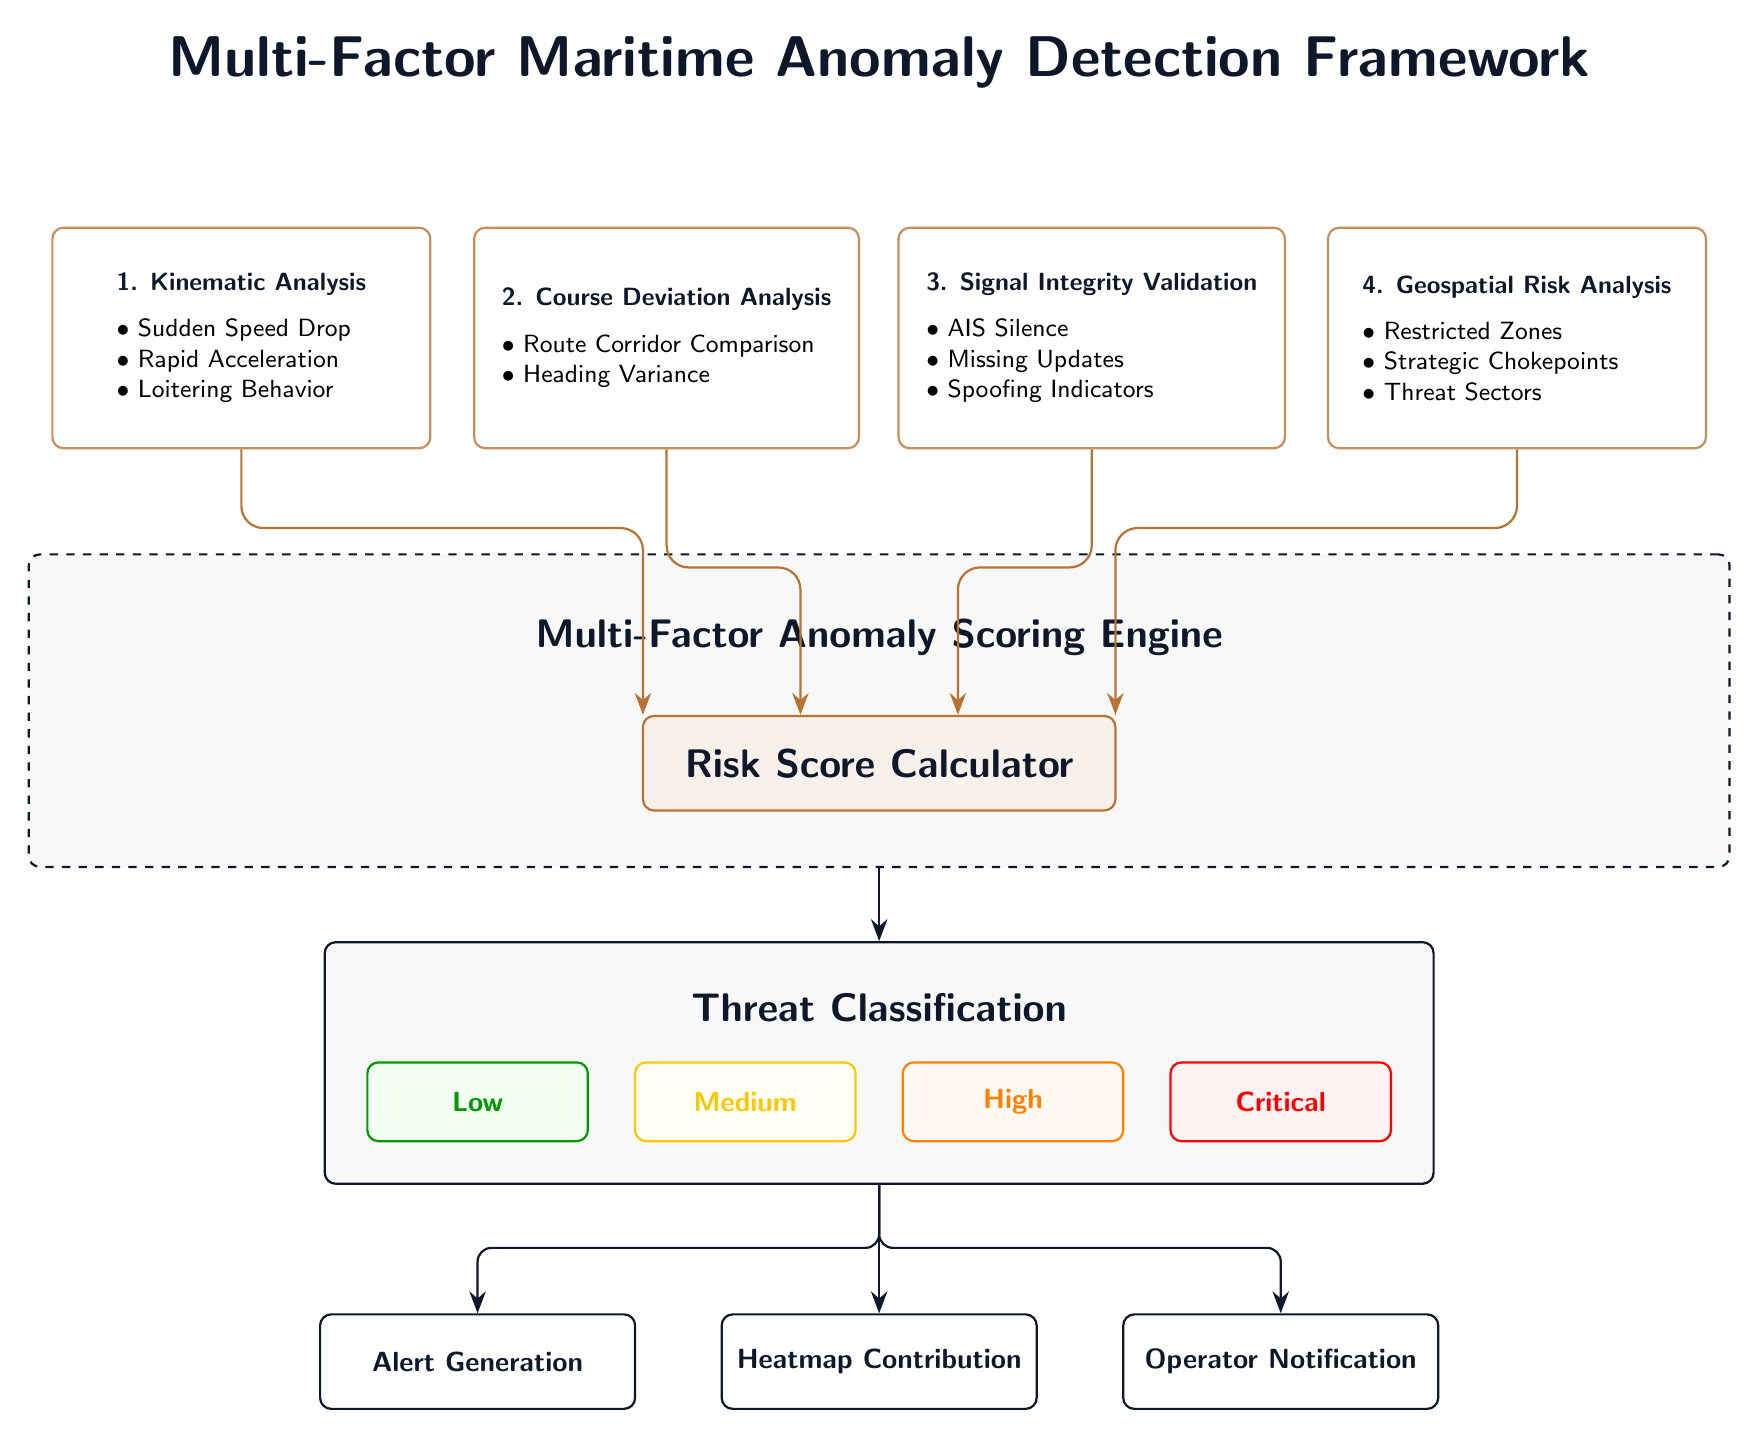
\begin{tikzpicture}[
    font=\sffamily,
    % Styles
    inputbox/.style={rectangle, draw=copper!80, thick, fill=white, rounded corners, minimum width=4.8cm, minimum height=2.8cm, align=left, font=\small, inner sep=10pt},
    calcnode/.style={rectangle, draw=copper, thick, fill=copper!10, rounded corners, minimum width=6cm, minimum height=1.2cm, align=center, font=\Large\bfseries\color{navyblue}},
    classbox/.style={rectangle, thick, rounded corners, minimum width=2.8cm, minimum height=1cm, align=center, font=\bfseries},
    low/.style={draw=green!60!black, text=green!60!black, fill=green!5},
    medium/.style={draw=yellow!60!orange, text=yellow!60!orange, fill=yellow!5},
    high/.style={draw=orange, text=orange, fill=orange!5},
    critical/.style={draw=red, text=red, fill=red!5},
    outputbox/.style={rectangle, draw=navyblue, thick, fill=white, rounded corners, minimum width=4cm, minimum height=1.2cm, align=center, font=\bfseries\color{navyblue}},
    arrow/.style={-{Stealth[scale=1.2]}, thick, navyblue},
    copperarrow/.style={-{Stealth[scale=1.2]}, thick, copper}
]

% ==================== TITLE ====================
\node[font=\huge\bfseries\color{navyblue}] (title) at (0, 8.5) {Multi-Factor Maritime Anomaly Detection Framework};

% ==================== INPUT PILLARS ====================
\node[inputbox] (in1) at (-8.1, 5) {
    \textbf{\color{navyblue} 1. Kinematic Analysis}\\[2mm]
    $\bullet$ Sudden Speed Drop\\
    $\bullet$ Rapid Acceleration\\
    $\bullet$ Loitering Behavior
};

\node[inputbox] (in2) at (-2.7, 5) {
    \textbf{\color{navyblue} 2. Course Deviation Analysis}\\[2mm]
    $\bullet$ Route Corridor Comparison\\
    $\bullet$ Heading Variance
};

\node[inputbox] (in3) at (2.7, 5) {
    \textbf{\color{navyblue} 3. Signal Integrity Validation}\\[2mm]
    $\bullet$ AIS Silence\\
    $\bullet$ Missing Updates\\
    $\bullet$ Spoofing Indicators
};

\node[inputbox] (in4) at (8.1, 5) {
    \textbf{\color{navyblue} 4. Geospatial Risk Analysis}\\[2mm]
    $\bullet$ Restricted Zones\\
    $\bullet$ Strategic Chokepoints\\
    $\bullet$ Threat Sectors
};

% ==================== CENTRAL ENGINE ====================
\node[font=\Large\bfseries\color{navyblue}] (engine_title) at (0, 1.2) {Multi-Factor Anomaly Scoring Engine};
\node[calcnode] (calc) at (0, -0.4) {Risk Score Calculator};

\begin{scope}[on background layer]
    \node[fit=(engine_title) (calc), rectangle, draw=navyblue, thick, dashed, fill=navyblue!3, rounded corners, minimum width=21.6cm, inner ysep=20pt] (engine) {};
\end{scope}

% Routing Inputs to Calculator
\coordinate (c1) at ($(calc.north) + (-3, 0)$);
\coordinate (c2) at ($(calc.north) + (-1, 0)$);
\coordinate (c3) at ($(calc.north) + (1, 0)$);
\coordinate (c4) at ($(calc.north) + (3, 0)$);

\draw[copperarrow, rounded corners=8pt] (in1.south) -- ++(0,-1) -| (c1);
\draw[copperarrow, rounded corners=8pt] (in2.south) -- ++(0,-1.5) -| (c2);
\draw[copperarrow, rounded corners=8pt] (in3.south) -- ++(0,-1.5) -| (c3);
\draw[copperarrow, rounded corners=8pt] (in4.south) -- ++(0,-1) -| (c4);

% ==================== THREAT CLASSIFICATION ====================
\node[font=\Large\bfseries\color{navyblue}] (class_title) at (0, -3.5) {Threat Classification};
\node[classbox, low] (low) at (-5.1, -4.7) {Low};
\node[classbox, medium] (medium) at (-1.7, -4.7) {Medium};
\node[classbox, high] (high) at (1.7, -4.7) {High};
\node[classbox, critical] (critical) at (5.1, -4.7) {Critical};

\begin{scope}[on background layer]
    \node[fit=(class_title) (low) (critical), rectangle, draw=navyblue, thick, rounded corners, inner sep=15pt, fill=navyblue!3] (class_fit) {};
\end{scope}

\draw[arrow] (engine.south) -- (class_fit.north);

% ==================== OUTPUTS ====================
\node[outputbox] (out1) at (-5.1, -8) {Alert Generation};
\node[outputbox] (out2) at (0, -8) {Heatmap Contribution};
\node[outputbox] (out3) at (5.1, -8) {Operator Notification};

\draw[arrow, rounded corners=5pt] (class_fit.south) -- ++(0,-0.8) -| (out1.north);
\draw[arrow, rounded corners=5pt] (class_fit.south) -- ++(0,-0.8) -| (out2.north);
\draw[arrow, rounded corners=5pt] (class_fit.south) -- ++(0,-0.8) -| (out3.north);

\end{tikzpicture}
\end{document}
